\section{Diseño}

\subsection{Diagramas de clases}

A continuación, mostramos un diagrama conceptual de clases que no representa la implementación final ya que incluye únicamente las clases más estrictamente relacionadas con el juego y la generación procedimental de contenido. También se han omitido métodos \textit{getter} y \textit{setter} por simplicidad.\\

\begin{figure}[H]
    \begin{center}
        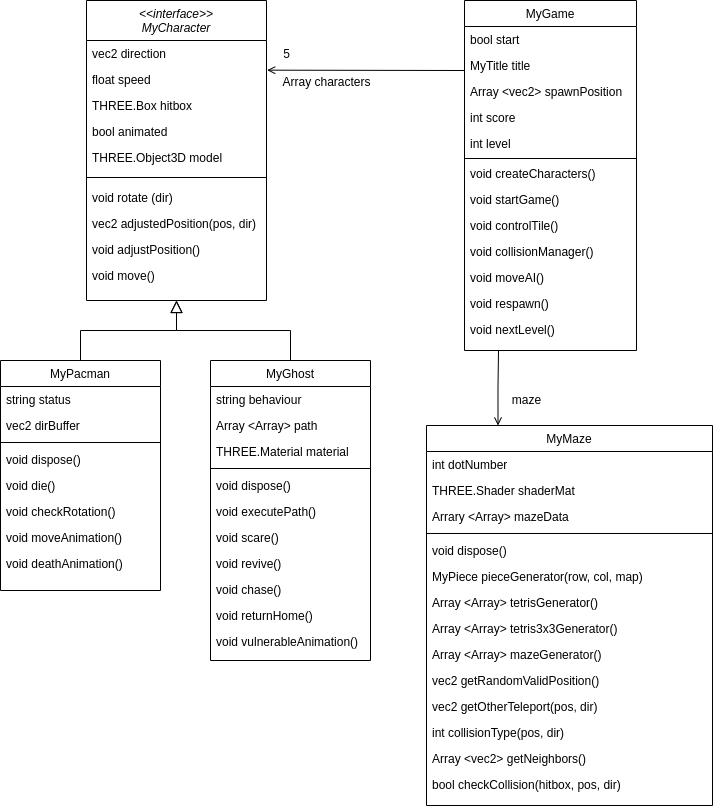
\includegraphics[scale=0.525]{img/clases.png}
        \caption{Diagrama simplificado de clases.}
    \end{center}
\end{figure}

% ---------------------------------------------------------------------------- %
\newpage
\subsection{Modelos jerárquicos}

Se ha decido crear manualmente los modelos de los personajes y siendo necesario de cara a crear animaciones como la del movimiento de la boca de Pac-Man, se ha creado modelos jerárquicos que representan las distintas partes y grados de libertad de los modelos \acrshort{3d} de nuestros personajes.\\

En el caso del modelo de Pac-Man, se trata de un modelo jerárquico con un grado de libertad compuesto de dos semiesferas, cada una de ellas acompañadas de una tapa que forma el interior de la boca.

\begin{figure}[H]
    \begin{center}
        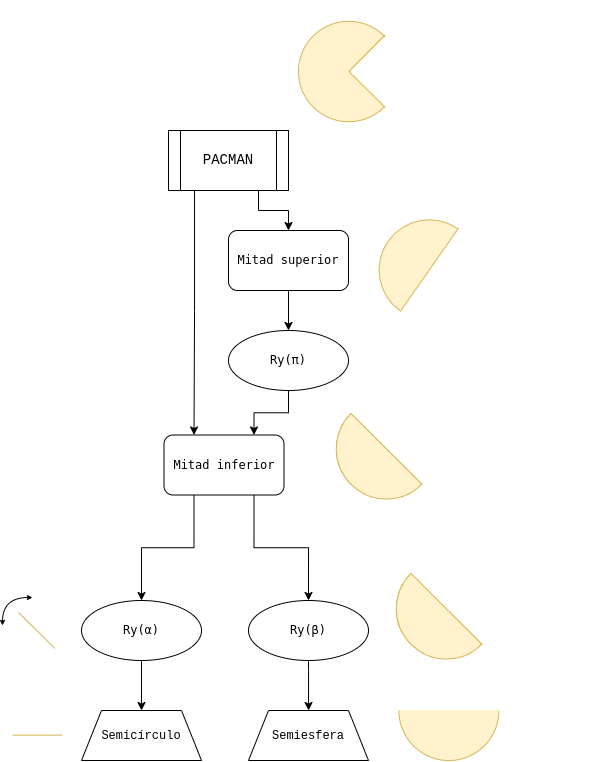
\includegraphics[scale=0.45]{img/pacman_jerarquico.png}
        \caption{Modelo jerárquico de Pac-Man.}
    \end{center}
\end{figure}

\newpage

En el caso de los fantasmas, aunque pueda parecer un modelo jerárquico más complejo, no cuenta con ningún grado de libertad ya que el modelo de los fantasmas es estático. El modelo está compuesto de una semi esfera y un cilindro que forman la cabeza y cuerpo de los fantasmas; cuatro esferas que forman los ojos; y 16 triángulos que, al colocarse alrededor de la base del fantasma, componen los pies de este.\\

Mencionar que los fantasmas utilizan como material los cuatro colores del juego original, rojo, rosa, naranja y azul claro.

\begin{figure}[H]
    \begin{center}
        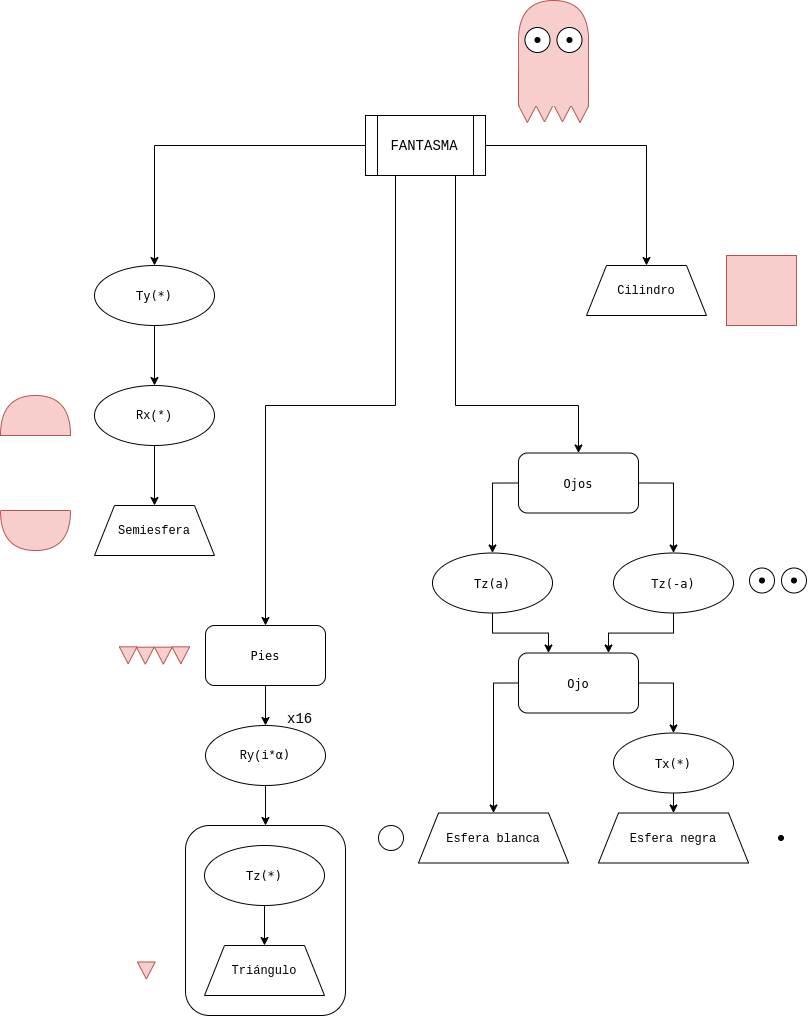
\includegraphics[scale=0.41]{img/fantasma_jerarquico.png}
        \caption{Modelo jerárquico de los fantasmas.}
    \end{center}
\end{figure}